\chapter{引言}
\label{cha:intro}

\section{论文的背景和意义}

2018年IPCC发布全球升温1.5摄氏度特别报告,报告指出,应该将全球变暖限制在1.5摄氏度以内,而过去的一个世纪,全球已升温约0.8摄氏度~\cite{globalWarming}。在全球变暖的背景下,寒潮、龙卷风、干旱、暴雨、暴雪和火灾等极端气候事件加剧。特别是近几年来,极端事件的频发,对人类的生命和财产都造成了不可挽回的损失。例如2016年我国暴雨频发,共出现46次区域暴雨,26个省(区、市)出现城市内涝;2017年非洲之角1月至2月严重的干燥季节以及3月至5月降雨极少的雨季,索马里超过半数的耕地遭受旱灾;2018年加利福尼亚遭受的毁灭性的野火是美国一个多世纪以来最致命的火灾。这些极端气候事件的出现,使得气候预测问题逐渐凸显对高精度预测日益迫切的需求。

气候系统模式是模拟气候状态中长期变化的数值模型,它通过构建一系列的数学物理方程组来近似模拟真实地球系统中存在的物理、化学和动力等复杂的过程以及地球各圈层之间的水汽、能量和物质的交换等,是预测未来气候的重要工具。它的发展要追溯到20世纪70年代中期,近40年来的研究集结了气象、物理、化学和计算机等多个学科的智慧~\cite{modelprogress}。从前期的只以地球流体为主要的模拟对象的各个分量模块的模拟发展到如今的大气、海洋、海冰、陆面等过程的耦合模拟。另外,随着气溶胶、大气化学、碳氮循环和人类活动等的加入,气候系统模式越来越庞大而精细。其物理过程在不断细化,模拟的分辨率也越来越高,运算代价极高,所需要的计算资源也随之增多,是典型的高性能计算应用。

%例如CESM(Community Earth System Model),世界上著名的气候系统模式之一,2度分辨率全球模拟的AMIP实验180进程,在intel最新处也需要约10小时。

气候系统预测的不确定性是导致气候模拟不准确性的主要原因。IPCC 第四次报告中指出其主要有温室气体等排放场景不确定性、气候系统内部变率不确定性和气候系统模式不确定性~\cite{hawkins2009potential}。IPCC 第五次报告中对排放场景的不确定性的处理是设计多个排放场景,在不同的场景下分别对气候进行预测~\cite{moss2010next},而内部变率的不确定性会随着模拟时间的变长而不断减小,所以目前亟待研究的关键问题是气候系统模式的不确定性。

而气候系统模式的不确定性又有初始条件不确定性和物理参数不确定性等。物理参数的不确定性指的是气候系统模式的次网格物理参数化过程中存在着大量的不确定性参数,这些参数是由专家根据经验而人为设定的。气候系统模式的每个模块中都存在着大量的不确定性参数,研究表明这些不确定性参数决定着模式模拟准确与否~\cite{mastrandrea2011ipcc}。初始条件的不确定性指的是气候模拟初始场的不确定性,因气候模拟存在典型的混沌特征,由洛伦兹提出的蝴蝶效应可知,初始场微小的差异将会引起混沌系统模拟结果的巨大差异,需要开展深入的研究工作来应对这些不确定性并改进气候预测能力。

从单一模块的气候系统模式到耦合气候系统模式,模式自身的不确定性也在不断攀升~\cite{stan2008influence,Evans2013A},针对高代价的不确定性大的耦合气候系统模式做不确定性量化工作是当前气候预测面临的重要问题之一。本文的主要思想是通过降低耦合气候系统模式的参数和初值不确定性来实现更高的气候预测能力。

\section{集合预测方法概述及相关工作}
\label{sec:first}
\subsection{集合预报思想}
集合预报技术由Epstein~\cite{epstein1969stochastic}和Leith~\cite{leith1974theoretical}首先提出,是量化不确定性,提升天气气候模拟水平的重要策略。1992年美国国家环境中心(NCEP)和欧洲气候预报中心(ECMWF)将数值天气集合预报系统投入业务运行。随后,日本、加拿大、中国等许多国家也分别建立了数值集合预报业务系统。但是由于气候系统模式运行代价极高的特性,气候集合预报相对于天气集合预报的研究还处于落后的状态。近年来,得益于高性能计算机的快速发展,气候集合预报也逐渐成为气候预测的重要手段。集合方法的原理是用多个集合预测代替原有的单一预测,利用多个集合成员所携带的大量信息进行天气气候定量预估。
集合预报的目的主要有以下两个方面:
(1)利用集合集成提高确定性预报的结果,当前常用方法是将多个集合成员结果进行集合平均,用平均的结果作为确定性预报结果,增强确定性预报的能力。(2)提供概率预报,分析各个集合成员的结果,计算气候事件出现的概率。通常气候集合预报的思路是对气候系统模式的控制预报进行扰动,得到多组扰动预报,将扰动预报结果和控制预报结果综合在一起得到最后的集合预报结果,集合预报概念示意图如图~\ref{fig:ensenature}所示。
\begin{figure}[H] % use float package if you want it here
  \centering
  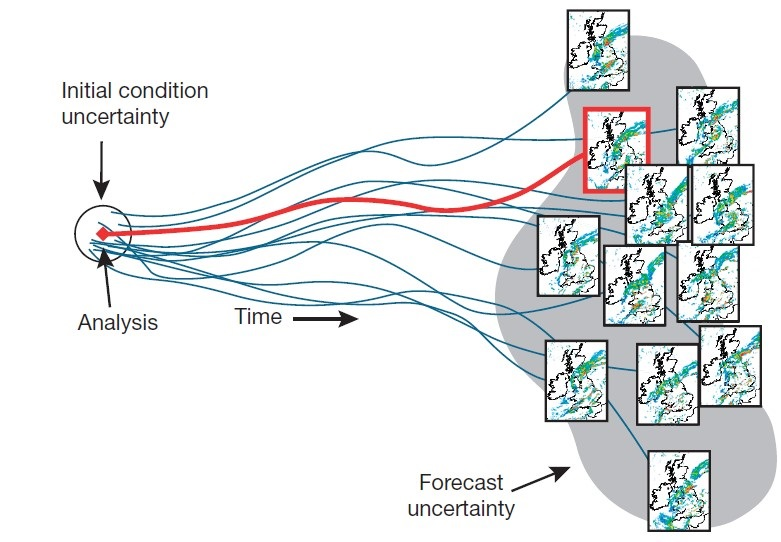
\includegraphics[scale=0.72]{figures/ensembleforecast_nature.png}
  \caption{集合预报概念示意图(摘自文献~\cite{bauer2015quiet})}
  \label{fig:ensenature}
\end{figure} 

\subsection{集合预报的扰动技术}
\subsubsection{初值扰动集合方案}
\label{sec:basictable}
气候系统模式的初值是由多个观测数据或者再分析资料同化得到的,其结果与真实的气候状态总是存在一定的差距。而气候系统模式又是典型的混沌系统,对于初始误差非常敏感。较小的初始误差在数值模拟的过程中,经过非线性叠加都会导致模拟结果具有非常大的差异。这也是著名的蝴蝶效应的由来。针对以上这两点,初值集合方法被用于天气和气候的预测当中。此方法的思想是从不同的初值状态开始启动预报,利用初值集合预报的结果来改善由于单一初值在混沌系统中形成的预测误差。现有的初值集合扰动方案大多数都是针对天气的,面向气候的集合技术研究还仍然在起步阶段。初值扰动方案获取扰动的基本原则有以下两个方面:一是要保证扰动场与用于预测的初始场的误差分布尽可能相似,这样才能保证每一个集合成员的初始场都有可能是真实的天气气候的初始状态,二是每一个扰动场在模式的模拟演进过程中,误差应该得以不断地发散,以保证集合成员最大可能包含实际的天气气候演进过程~\cite{陈静2002集合数值预报发展与研究进展}。

\subsubsection{模式扰动集合方案}
气候系统模式是由动力框架和物理过程共同组成的,次网格尺度的物理过程多是由统计分析得到,每个分量模式的物理过程也是在不断的发展中。模式结构的不确定性催生了模式扰动集合方案。通常的集合方法有:在模式的非绝热强迫项中加入随机噪声~\cite{buizza1999stochastic,berner2009spectral}以及选择不同的物理参数化方案作为集合成员~\cite{houtekamer1996system}等。研究表明,当前模式扰动集合方案最多的还是参数化方案的扰动,而参数化方案的个数毕竟有限,所以通常模式扰动集合方法需要配合初值扰动集合方案一起使用。

\subsection{多模式扰动的超级集合方案}
因单一气候模式在各种气候问题的表征上难以都达到行业前沿的水平,因此目前国际上也在设计多模式扰动集合预报系统以吸收多个优秀气候系统模式的优点~\cite{mylne1999quasi,evans1997joint}。但是相对于单一气候系统模式而言,多模式集合扰动的理论和技术方法还不够成熟,且在长期气候模拟上,多模式集合预报所需要的计算资源更多,计算代价更高。

\subsection{集合预测面临的问题及已有工作}
针对复杂气候系统模式的集合预测技术研究存在着巨大的挑战。主要有以下几个方面:

1. 气候系统模式中不确定参数问题严峻。气候系统模式由不确定性参数而导致的性能变化是多峰,非线性极强的空间~\cite{zhang2015automatic}。IPCC第五次报告中指出仅由参数不确定性变化而导致的气候系统模式模拟的全球平均温度差异可以达到2摄氏度左右。为了准确地模拟气候状态,对气候系统模式进行参数不确定性分析是十分重要的环节。

现有的不确定性分析方法主要分为前向的不确定性分析和反向的不确定性分析。下面将对这两类方法分别介绍。

前向的不确定性分析方法其核心思想是通过设计实验以及定量分析结果的统计特征等增加对问题本身的了解。主要的方法有采样、敏感性分析、构建代理回归模式等等~\cite{neelin2010considerations}。在不确定参数空间中进行采样,通过对采样点的评估,估计参数后验分布可能的情况。其方法可以是蒙特卡罗采样,单参数扰动采样,拉丁超立方采样,以及自适应采样等。敏感性分析是指通过对参数的扰动来获取参数的灵敏度信息,如果一个参数扰动极小的幅度就会对评估结果产生较大的影响,那么就可以判定其为敏感参数。敏感性分析方法主要分为局部敏感性分析和全局敏感性分析。局部敏感性分析主要考虑的是参数的一阶效应。不考虑两个或多个参数之间的交互效应。而全局敏感性分析是要同时考虑一阶效应和交互效应的~\cite{saltelli1995sensitivity,song2015global}。一般在气候系统模式中参数之间的交互效应是极强的。构建代理模式是利用统计回归等方法构建类似原来复杂问题的简单模型,用简单模型代替复杂模型的运行~\cite{xu2018parameter,muller2015ch4}。

反向的不确定性分析方法不考虑问题的统计特征,不要求对问题的后验分布有很好的了解,主要是将每一次模型的运行结果与观测进行对比,用对比结果来指导下一次参数的取值。主要的方法是数值优化方法。数值优化方法有传统的优化方法和进化优化方法等。传统的数值优化方法有单纯形下山方法、鲍威尔(powell)方法等,这些方法是局部优化方法,其特点是优化速度很快,能够快速收敛,但是在复杂多维的问题下容易陷入局部最优~\cite{severijns2005optimizing}。进化方法通过模拟种群进化的策略来不断更新样本,在种群中,根据物竞天择,适者生存的进化理论,只有表现好的样本能够以较大概率保留其基因到下一代。进化算法种类很多,例如协方差自适应调整进化策略(CMA-ES),差分进化(DE)等。它们主要的特点是克服陷入局部最优解的能力变强,但是需要的迭代次数也更多了,收敛性变差~\cite{auger2012tutorial,Storn1997Differential}。

上述提到的方法大都数都是为小应用而设计的,对小应用进行参数不确定性量化时对问题迭代多次求解,在时间和计算资源上也是可以接受的,但是像气候系统模式这种大应用,一次迭代需要很长时间,成百上千次的模拟显然在计算资源和时间上都难以接受。计算代价高的应用的不确定性分析对算法的性能和收敛性都提出了更高的要求~\cite{zhang2015automatic}。

2. 面向气候预测的初值集合扰动方法研究欠缺。初值扰动集合方法在天气预报中的应用已趋向成熟,但是针对更加复杂的气候系统模式来说初值集合预报方法还处在起步阶段。

通常用于天气预报的初始扰动集合方法包括蒙特卡罗随机方法、滞后平均法、奇异向量法和增长模繁殖法等。蒙特卡罗随机方法是对于初值做随机的微小扰动,用扰动后的初值分别进行模拟得到不同的模拟结果,其主要的缺点是随机扰动可能与真实初始场的误差并不相符,不好把握扰动的力度。滞后平均法获取初值扰动的方法是通过将从起报时间往后滞后若干天,例如第一个集合是起报日期,第二个集合就是起报日期往前推3天,第三个集合就从起报日期往前推6天,其他的集合起报日期依次类推。滞后平均法主要是利用了相近时间天气的状态相似性来组成了多个近似的初值扰动~\cite{hoffman1983lagged}。

蒙特卡罗随机和滞后平均法(LAF)实现相对简单,但是都缺乏较强的理论基础。在此基础上奇异向量法(Svs)和增长模繁殖法(BGM)方法相继被提出。奇异向量法由Buizza和Palmer首先提出的,该方法使用切线模型及其伴随向量计算奇异向量。用最大奇异值对应的奇异向量作为增长最快的扰动。该方法从1996年开始在欧洲中期天气预报中心得到使用~\cite{molteni1996ecmwf}。BGM是方法是Kalnay和Toth提出的,此方法在客观分析场上叠加随机扰动,进行预报,将控制预报减去扰动预报的差值调整后,作为下一次计算的扰动量,如此循环反复使用,最终形成初始场。此方法提供了对最快的可持续增长误差的估计,并代表了误差进展的可能方向~\cite{toth1997ensemble}。

尽管BGM和SVs集合方法在天气预报中得到广泛的应用,但它们很少用于气候预报。主要原因是SVs方法生成初始扰动的方法十分复杂,一般需要用到伴随模式,且在气候系统模式中需要极高的计算资源。而BGM方法由于高频噪声增长速度过快,导致增长模的增长率快速达到饱和,无法完全捕获气候系统模式中的一些慢变化过程的特征。因此,在许多国际前沿季节气候预报系统,如NCEP气候预报系统第2版(CFSv2)~\cite{saha2014ncep}以及北京气候中心的季节预报~\cite{liu2014relationships}中的集合策略仍然使用滞后平均法(LAF)。但是由于气候一直处在一个动态变化的过程中,对于初始场误差的表征仅仅用之前的状态来作为扰动显然是不够的。

%近几年,针对亚季节到季节时间尺度的气候预测集合方法的研究相继出现。 Kug等人。 (2010)将经验SVs方法应用于混合耦合模型的ENSO预测,并表明该方法可用于CGCM中的季节预测~\cite{kug2010new}。 Johanna和Piontek表明,与LAF方法相比,在ECHAM5 / MPIOM耦合气候系统模型的模拟中,在海洋组件中实施BGM可以改善温度和盐度的集合扩散~\cite{}。在Hudson等人的研究中。 (2013)和Kang等人。 (2014),通过在气候系统模型的季节预报系统中使用育种方法,改进了Madden-Julian Oscillation(MJO)的预测技巧。
%
气候系统模式本身的复杂度很高,加上集合也是高计算代价的策略,对于气候系统模式集合方案的研究进展相对缓慢。目前的初值集合方案大多数是针对天气模式建立的,在气候系统模式中如何提高集合模拟精度的问题一直存在。


3. 集合集成方法有待改进。因为集合预报多个成员的预报结果有一定的离散度,各个成员的预报分布并不相同,另外由于气候系统模式的系统偏差等原因,集合预报集成结果改进的空间很大。

当前确定性集合集成最常用的方法仍然是集合平均的方法。然而在气候系统业务预报中通常每月都会开始启动向前几个月的气候预测,每次有多个集合成员。如此众多的信息如果只用来做集合平均的话对计算资源是一种浪费。针对这一问题,基于模型数据和观测数据融合的集合集成技术正在悄然发展。其主要思路是将模式的输出结果与观测结果做对比,找出模式出现偏差的趋势,在真正做预测的时候将模式预测结果去掉这个趋势。常用的方法有概率匹配平均法,相似度集成法,最优百分位集成法等。

概率匹配法是将各个成员的空间分布按照优劣排序,空间分布结果越好的其集合权重系数越高,反之权重系数越低~\cite{ebert2001ability}。相似度集成法是将各个集合成员的空间分布的相似性作为评价标准,相似性越高则成员权重系数越高~\cite{陈力强2005短期集合预报中定量降水预报集合方法初探}。最优百分位法是利用历史数据提高不同等级的集成结果。例如不同降水等级有不同的集合成员及其权重系数~\cite{代刊2016中短期数字化天气预报技术现状及趋势}。

由此可见当前的集合集成方法多为统计分析法,随着集合成员数的增多,模式模拟时长的增加,更多的气候数据被积累,数据量越来越大,此时传统的集成方法就力有不逮,不能充分的使用已有数据。所以集合集成方法需要进一步改进。

\section{本文研究的主要内容}
\subsection{本文的研究内容和主要贡献}

针对当前气候预测中集合预报技术面临的问题,本文设计了一种结合参数优化的初值集合方案,其主要流程是针对气候系统模式的参数不确定性对物理过程中的参数进行优化,利用优化参数后的模型为集合预报打下良好的基础。在改善后的模型上设计了初值不确定性方案,并进一步开展集合集成技术的研究以改进确定性预报的性能。本文的主要研究内容和贡献有以下几个方面:

1.面向气候系统模式的高效参数优化方法。本文针对气候系统模式的高计算代价和强非线性等特点设计了基于多层感知机神经网络的代理模式参数优化方法:利用代理模式来估计下一个最优采样点,每增加一个采样都更新寻优策略。该方法相比进化优化算法的种群更新策略能够使得优化过程计算量更小,收敛速度更快,而相对于基于传统统计回归代理方法的模型,基于多层感知机神经网络的代理模式更适合复杂问题代理模型的构建。另外本文利用此优化思路构建了单目标优化算法、多目标优化算法和有约束优化算法并在复杂数学函数和单柱大气模式的优化试验中验证了所提出算法的有效性。

2. 面向气候预测的初值集合方案设计。针对气候系统模式初值集合方案存在的问题,设计了基于增长模繁殖法的集合方案,并对比了该方案与国家气候中心现用的LAF方法的预测效果。基于BCC-CSM(Beijing Climate Center Climate System Model)模式的对比结果显示,新设计的BGM方案比原方法在第一个月的性能提升非常显著。

3.结合参数优化的初值集合方案设计和应用。结合参数优化和初值集合方案,本文设计了一种面向气候预测的BGMOPT集合方法,并将其在BCC-CSM模式2008年12月至2009年3月的降雨预报中与原LAF方法进行对比。结果表明此方法在降雨预测中比原LAF方法更优。

4. 基于机器学习的集合集成技术研究。确定性预报需要对集合成员的结果做集成,但是现在最常用的气候预测集成方法还是集合平均法,本文设计了一种基于机器学习的集成技术,此技术利用了观测数据和已有模式输出的大量数据对模式集合预测结果进行集成修正。修正后的模式预测能力相对原集合平均法改进32\%。

5. 气候集合预测系统设计与实现。综合以上内容,本文设计了面向气候的集合预测系统。此系统中包括了不确定参数的优化、初值扰动方案的设计、集合预测的模拟过程、集合结果集成修正等模块,实现了自动化的气候预测与结果分析。

\subsection{本文的组织架构}
本文共5个章节,每一章的具体内容如下:

第1章首先介绍了研究背景和意义,简述了气候系统模式的工作原理及其发展历程,然后介绍了集合预报的概念及其常用方法。最后针对气候系统模式集合预测存在的问题展开讨论并总结了已有的工作。

第2章首先介绍了气候系统模式参数优化问题,然后描述了各类问题的当前常用方法和本文提出的方法。并将常用方法和本文方法在单柱大气模式和复杂数学函数上进行了测试和对比。最后介绍了各类优化算法的整合和简要的实现过程。

第3章首先介绍了当前面向气候的集合初值扰动方案存在的问题。然后介绍了天气中的常用的初值集合方法BGM的流程,并解释了为何它不适用于气候系统模式。然后针对气候预测的特征,重新设计了面向气候预测的BGM方法,并将其与国家气候中心所使用的LAF在BCC-CSM模式上做了对比。

第4章首先介绍了本文所提出的结合参数优化的初值集合方法,然后针对当前集合集成方法未能充分应用大量已有模式输出数据和观测数据的问题,提出了基于机器学习的集合预测修正技术,最后本文描述了包含自动参数优化、初值扰动生成、集合预报、集合集成等模块的综合集合系统设计与实现,并叙述了该系统在BCC-CSM模式上的应用案例。

第5章是全文的总结,并提出了下一步工作的方向。